\subsection{iOS}\label{sec:components-syssec} 
	Eine Kette von aneinander gereihten und von einander abhängigen Prozessen trägt
	maßgeblich zur Systemsicherheit von iOS bei. Dies berücksichtigt vor allem den
	Startvorgang, die Softwareupdates - auch von Drittanbietern - und den Secure
	Enclave (Kapitel \ref{sec:secure_enclave}). Dies stellt sicher, dass
	alle Kernkomponenten, ob Hard- oder Software, möglichst gefeit vor Angriffen sind,
	ohne dabei die Nutzerfreundlichkeit zu beeinflussen. Wenn dabei einer dieser
	Schritte fehlschlägt, unterbricht der Startvorgang und das Gerät wird in den
	Recovery Modus versetzt. Wenn der Boot-ROM nicht geladen werden kann, wird der
	DFU\footnote{DFU: Device Firmware Upgrade - Modus zum Upgraden von USB-Geräten}
	Modus betreten.\\
	Nachfolgend werden die Komponenten, welche maßgeblich zur Wahrung der
	Systemsicherheit und der Integrität dieser beteiligt sind, detailliert
	vorgestellt und beschrieben.
	
	\begin{figure}[h]
		\centering
		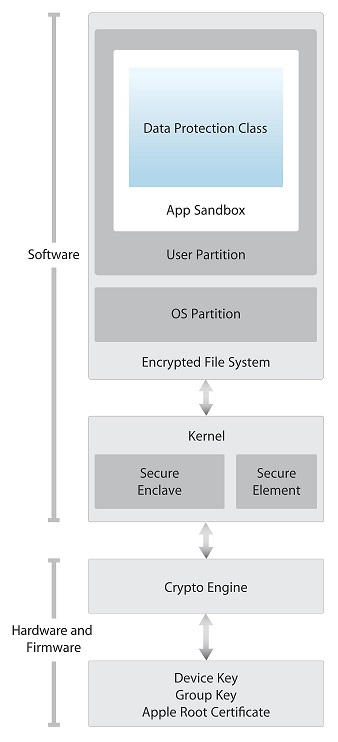
\includegraphics[width=0.4\linewidth]{ios/media/security-model.jpg}
		\caption{Sicherheitsmodel von iOS 
		\cite[S.4]{iOSSecurityApr2015}}
		\label{fig:security-model}
	\end{figure}

	\subsubsection{Secure boot chain}\label{sec:secure-boot-chain}
		Dieses Verfahren stellt eine Manipulation der Software auf niederer
		Systemebene sicher.
		Nur iOS Geräte, deren Vertrauenskette erfolgreich validiert wurde, starten
		ordnungsgemäß. Dabei wird nach dem Start eines iOS Gerätes zuerst Code aus
		einem nur lesbaren Speicherbereich gelesen. Dieser \textit{hardware of
		trust} genannte und unveränderbare Code ist bei der
		Manufaktur der Chips eingebettet worden und somit implizit vertraulich.
		Er enthält das Wurzelzertifikat von Apple, einen gerätespezifischen
		Schlüssel (UID\footnote{UID: Unique ID - pro iOS Gerät und Prozessor einzigartiger,
		in Hardware gegossener 256-Bit AES Schlüssel}) und einen Gruppenschlüssel
		(GID\footnote{GID: Group ID - ein 256-Bit AES Schlüssel der allen
		Prozessoren einer Klasse (vgl. Kapitel \ref{sec:filesecurity}) bekannt ist}).
		Das Wurzelzertifikat stellt eine Signierung des Low-Level-Bootloaders durch Apple sicher, bevor er ausgeführt wird.
		Dies ist der erste Schritt in der "`chain of trust"', in welcher jeder
		Teilnehmer sicher stellt, dass der darauf folgende von Apple signiert ist. 		
		Nach erfolgreicher Abarbeitung aller Aufgaben des LLB, überprüft und startet
		dieser iBoot, den nächsten Bootloader, welcher wiederrum das selbe Prozedere
		mit dem iOS Kernel beginnt. Bei Geräten mit Mobilfunk Zugang führt das
		Basisband Untersystem seinen eigenen ähnlichen Prozess mit signierter 
		Software und verifizierten Schlüsseln des Basisband Prozessors durch.
		
	\subsubsection{Authorisierung von System Software}\label{sec:code-signing}
		Dieser Prozess soll einen Downgrade auf eine ältere Version von iOS
		verhindern und benötigt eine Internetverbindung. Der in Kapitel
		\ref{sec:secure_enclave} besprochene Secure Enclave Co-Prozessor nutzt diese
		Technik ebenfalls für die Integritätsprüfung seiner Software. Im Falle eines
		iOS Updates wird entweder von iTunes oder ab iOS 5 vom Gerät selbst
		(OTA\footnote{OTA: Over The Air}) einer der autorisierenden
		Installationsserver von Apple kontaktiert. Dieser erhält eine Liste mit
		verschlüsselten Informationen für jede Komponente, die am Update beteiligt
		ist.
		Zusätzlich wird ein zufälliger Anti-Replay Wert und die UID des Gerätes
		verschickt. Die Clientdaten werden gegen eine Auflistung authorisierter
		Hardware geprüft, für die ein Update genehmigt ist. Bei
		Übereinstimmung wird die eindeutige ECID\footnote{ECID: Exclusive Chip ID - eine einzigartige
		64-Bit ID auf jedem iOS Gerät} zu den Informationen ergänzt und das
		Ergebnis signiert, was einer Personalisierung der Daten gleicht.
		Anschließend werden alle nötigen Daten vom Server signiert und zum Gerät
		geschickt. Die sichere Startkette von Prozessen (Kapitel
		\ref{sec:secure-boot-chain}) verifiziert die Signatur der empfangenen Daten
		auf den Absender Apple und startet anschließend einen Prüfsummenabgleich
		der empfangenen Daten.\\
		Mit diesen Schritten wird eine Authorisierung ausschließlich für freigegebene
		Geräte sicher gestellt. Außerdem verhindert der Anti-Replay Wert ein
		Manipulieren der Serverdaten, oder ein Mitschneiden dieser für
		das Verwenden auf anderen, nicht authorisierten Geräten.
		
	\subsubsection{Secure Enclave}\label{sec:secure_enclave}
		Dieser Co-Prozessor kommt in Geräten mit A7 oder jüngeren A-Serien
		Prozessoren - ab dem iPhone 5s - vor. Er verwendet seinen eigenen
		sicheren Startvorgang, ist separiert vom Applikationsprozessor und verwendet
		verschlüsselten Speicher, sowie einen Hardware Zufallszahlen Generator. Die
		Technologie basiert auf ARM's TrustZone \cite{TrustZone2015} und wurde von
		%TODO: vergleich auf android mit tee
		Apple für die eigenen Ansprüche angepasst. Der Kernel dieser Einheit basiert
		auf der L4 Mikrokernel-Familie \cite{L4MicroKernel2015} mit leichten
		Modifikationen. Die auf Interrupts basierende Kommunikation zwischen dem
		Applikationsprozessor und dem Secure Enclave wird über einen
		ausschließlich beiden Parteien zur Verfügung stehenden Speicherbereich
		abgearbeitet. Der SE\footnote{SE: Secure Enclave - Co-Prozessor von iOS
		Geräten ab A7 Chipsatz} ist verantwortlich für das Schlüsselmanagement der
		Datenverschlüsselung und stellt die Integrität dieser sicher, auch wenn der
		Kernel des iOS Systems kompromitiert ist. Beim Herstellungsprozess erhält
		jeder SE, wie der Applikationsprozessor eine einzigartige gerätespezifische
		ID (UID) und Gruppen-ID (GID), auf welche nur er zugreifen kann (vgl. Kapitel
		\ref{sec:secure-boot-chain}).
		Selbst Apple, oder anderen an der Produktionskette beteiligten Herstellern
		ist diese unbekannt. Mit dieser UID wird beim
		Systemstart der Speicherbereich des SE zusammen mit einem einmaligen
		Schlüssel chiffriert.
		Zusätzlich werden jegliche vom SE in den Speicher geschriebene Daten mit der
		UID und einem Anti-Replay Zufallswert verschlüsselt. Eine der Hauptaufgaben
		des Secure Enclave ist die Verarbeitung der Fingerabdruckdaten des Touch ID
		(Kapitel \ref{sec:touch_id}).
		Jegliche Kommunikation zwischen Touch ID und SE wird über einen seriellen Bus
		abgearbeitet. Der Applikationsprozessor leitet die Fingerabdrucksdaten an den
		SE weiter, kann diese aber aufgrund einer Verschlüsselung der Daten mit einem
		Sitzungsschlüssel nicht lesen. Dieser Session Key wird durch einen
		für Touch ID und SE vom System bereit gestellten öffentlichen
		Schlüssel erzeugt. Der Austausch des Sitzungsschlüssels wird durch
		AES\footnote{AES: Advanced Encryption Standard - ein symmetrisches
		Verschlüsselungsverfahren} Key Wrapping\footnote{Key Wrap - symmetrisches
		Verschlüsselungsverfahren zum Ummanteln von Schlüsseln} realisiert. Dabei
		erzeugen beide Seiten einen zufälligen Schlüssel, welche gemeinsam den
		Sitzungsschlüssel bilden. Zum verschlüsselten Transport wird
		AES-CCM\footnote{CCM: Counter with CBC - ein Verfahren, um Blockchiffren
		zusätzlich mit Integrität zu versehen} genutzt.
		
	\subsubsection{Touch ID}\label{sec:touch_id}
		Touch ID bezeichnet den Fingerabdrucksensor der in allen iPhone 5s und neuer
		, sowie iPad Air 2 und iPad mini 3 verbaut ist. Es können bis zu 5
		Fingerabdrücke gespeichert werden. Einer der größten Vorteile ist das
		sofortige Sperren des Gerätes beim Drücken des Sleep/Wake-Buttons.
		Hintergrund hierzu: vor der Einführung von Touch ID haben viele Nutzer eine
		möglichst lange Zeit eingestellt, bis das Eingeben des \textsl{passcode}\footnote{passcode -
		Passwort für den Zugang zu einem iOS Gerät, entweder simple (4 Zahlen), oder
		komplex ((Sonder-)Zeichen und Zahlen)} nötig war, nachdem das Gerät gesperrt
		wurde. Dies entfällt nun bei aktivierter Touch ID, da der Nutzer nur noch mit
		seinem Finger Entsperren muss.
		Touch ID kann zusätzlich zum Entsperren des Gerätes, mit dem Zahlungsdienst
		Apple Pay und für Einkäufe in iTunes, dem App Store und im iBook Store genutzt
		werden. Für Entwickler steht eine API bereit mit der rudimentärste
		Prüfungen auf erfolgreiche Verifikation des Abdrucks erfolgen können. Ein
		direkter Zugriff auf Touch ID oder die Daten des Fingerabdrucks wird von
		Apple unterbunden. Touch ID wird aktiviert, wenn der kapazitive Stahlring um
		den Sensor einen Fingerdruck wahrnimmt. Anschließend wird dieser gescannt und
		an den Secure Enclave gesandt. Der Abdruck wird kurzzeitig im veschlüsselten
		Speicher des SE für eine Vektorisierung\footnote{Vektorisierung - Konvertieren
		von Rastergrafiken in Vektorgrafiken} der Fingerabdruckdaten gespeichert, um
		danach verworfen zu werden.
		Die Schlüssel, welche von Touch ID zum Entschlüsseln des Gerätes benötigt
		werden, sind nach 48 Stunden ungültig, beziehungsweise wenn das iOS Gerät neu
		gestartet wurde, oder der Fingerabdruck fünf mal falsch registriert wurde.
		%TODO: double check this
		Danach muss der passcode des Systems erneut eingegeben werden.\\
		Dass diese Technik nicht als Sicher angesehen werden darf, haben bereits
		Miglieder des Chaos Computer Club gezeigt \cite{CCCBreakTouch2015}, dabei 
		wurde mit simpelsten Haushaltsmitteln ein Fingerabdruck gefälscht, den das
		Smartphone irrtümlicher weise akzeptiert hat.
